\subsection{Fravælgelse af gestik-par}
\label{TestresultaterPauseStartDaarlig}
%
I følgende afsnit analyseres hvilke af de syv semaforiske gestik-par testpersonerne fravælger samt hvorfor testpersonerne netop fravælger disse gestik-par. På baggrund af analysen bør det være muligt at udpege hvilke semaforiske gestikker, der hvertfald ikke skal knyttes til hverken pause eller start. Analysen bygger på testpersonerne respons til spørgsmålet: \textit{Hvilken gestik kan du mindst lide? og hvorfor?}, hvor testpersonernes samlede data er vedlagt i ELEKTRONISK BILAG.
%
\begin{figure}[H]
	\centering
	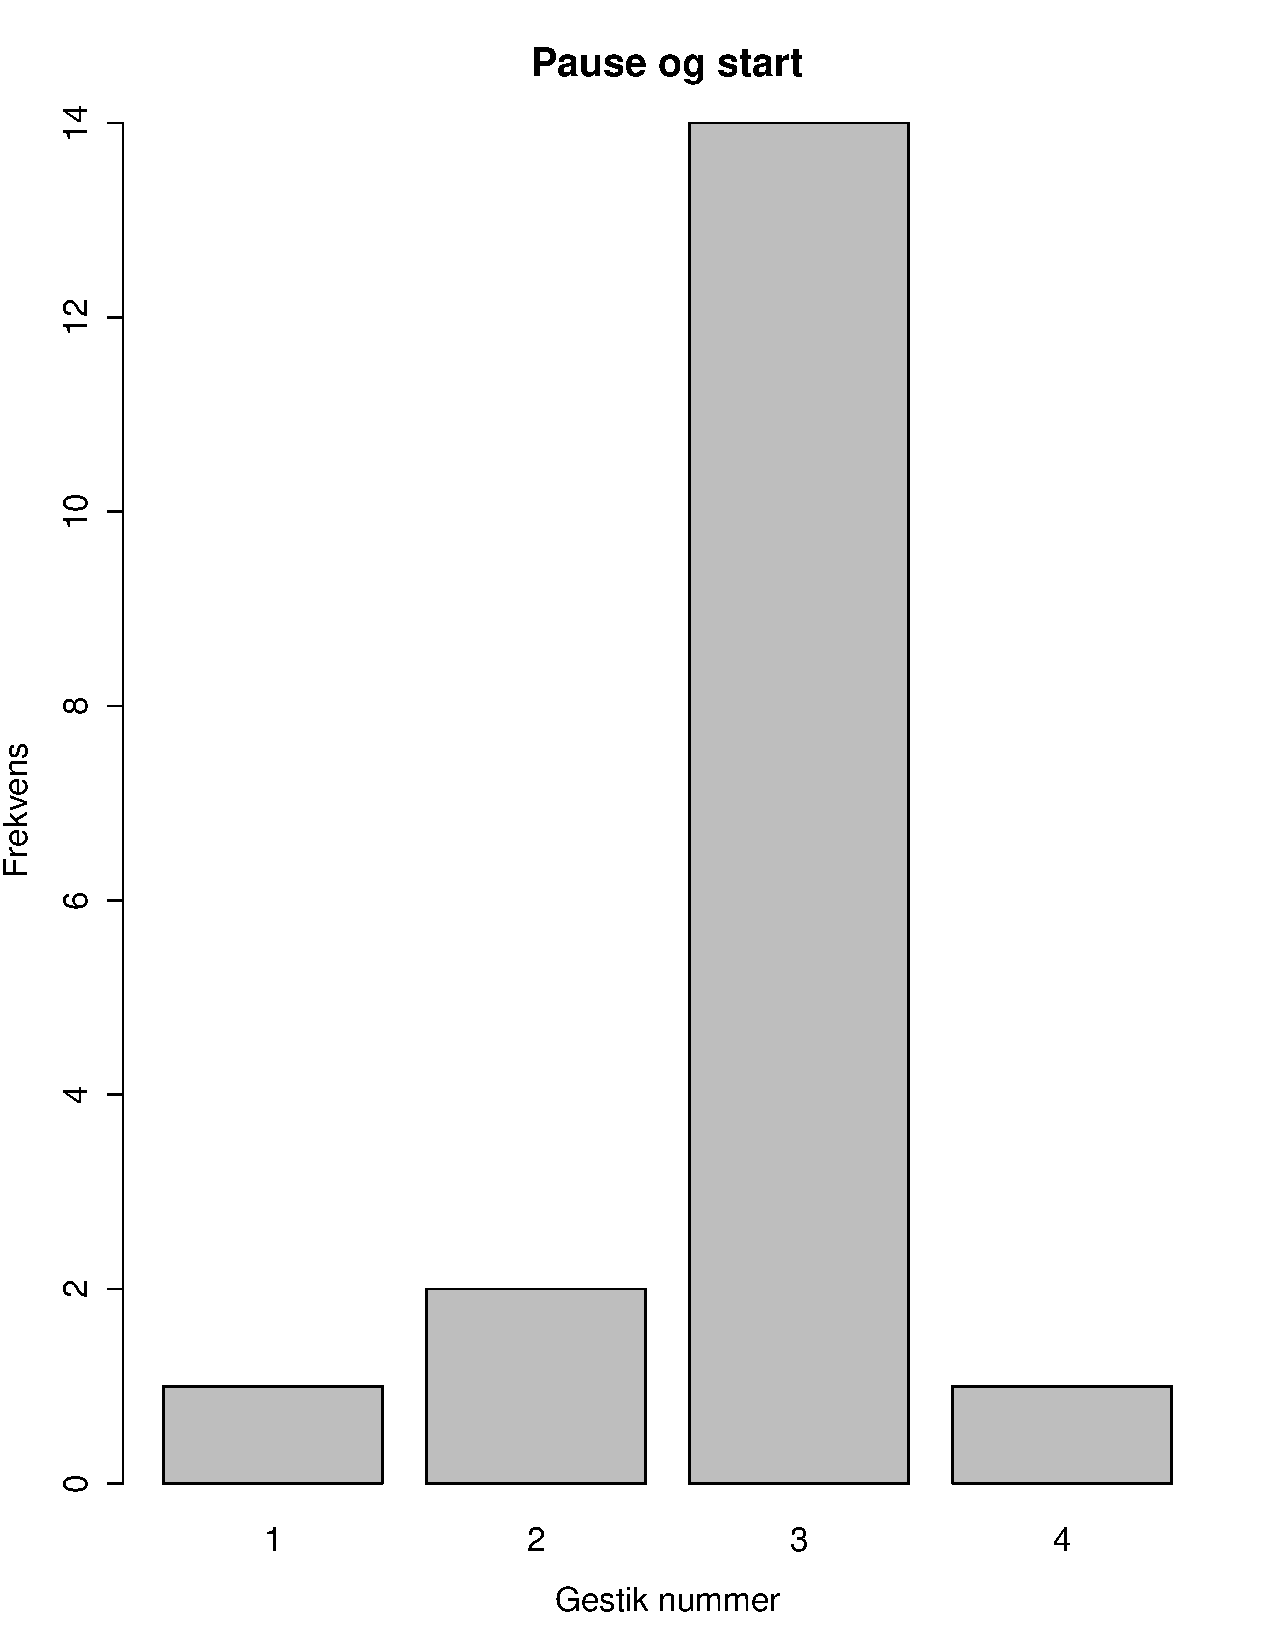
\includegraphics[resolution=300,width=0.5\textwidth]{Test1/DatabehandlingGrafer/DaarligstGestikPause.pdf}
	\caption{Barplot over hvilke gestik-par testpersonerne fravælger i forbindelse med pause og start. Søjlerne bygger på testpersonernes respons, hvorfor det kun er de fravalgte gestik-par, der udgør plottet.}
	\label{fig:DaarligstGestikPause}
\end{figure}
\noindent
% 
På \autoref{fig:DaarligstGestikPause} fremgår det hvilke gestik-par de 18 testpersoner fravælger i forbindelse med at skulle pause og starte musikken. Det fremgår tydeligt at gestik-par 3 er det par, som flest testpersoner fravælger i forhold til de tre andre gestik-par, der ellers er repræsenteret på \autoref{fig:DaarligstGestikPause}. Gestik-par nummer 1 fravælges af én testperson, testperson 13, fordi testpersonen forbinder det med at række en hånd i vejret. Testperson 1 og testperson 8 fravælger gestik-par 2 på baggrund af bevægelsesmængden, hvor begge testpersoner giver udtryk for, at der er for meget unødvendig bevægelse. Årsagen til at testperson 5 fravælger gestik-par 4 skyldes at testpersonen generelt ikke bryder sig om at pege. I og med at testperson 5 både kommenterer at den er lidt aggressiv og at det vil føles lidt mærkeligt at stå derhjemme og pege, så tyder det på at testpersonen oplever gestik-par 4 som værende social uacceptabel. 

De resterende 14 testpersoner fravælger alle gestik-par 3. De to største årsager til at parret fravælges er på grund af kompleksiteten i bevægelsen og at det simpelthen er for besværeligt at udføre. I forhold til bevægelsen giver flere testpersoner udtryk for at den, foruden at være kompleks, enten er for underlig, testperson 3, for mærkelig, testperson 4, for lang og akavet, testperson 7 og for indviklet, testperson 12. I tillæg kommenterer testperson 17, at det bliver en større øvelse at skulle pause og starte musikken, og så vil der gå langtid før musikken rent faktisk bliver sat på pause. Derudover giver testperson 14 og testperson 15 udtryk for at det ikke er sikkert, at de kan huske hvordan bevægelsen er. I tillæg kommenterer testperson 14 at hun simpelthen ikke ville vide hvordan hun skulle tænde eller slukke for lyden, svarende til at sætte musikken på pause og starte den igen. Testperson 9 giver udtryk for lignede bekymringer for hvordan musikken sættes på pause og startes igen.

Af de 18 testpersoner, der har deltaget i testen, er der kun to, som har inkluderet gestik-par 3 i deres rangering, det er testperson 8 og testperson 13. Begge testpersoner vælger gestik-par 3 som deres første prioritet, lige ind til at testperson 8 til sidst skal gengive de fortrukne gestikker og ind til testperson 13 skal lave en forbedring, hvorefter parret, i begge tilfælde, rangeres, som den næste bedste. Årsagerne til at testperson 8 har inkluderet gestik-par 3 blandt de tre bedste er dels at den er unik, speciel og sjov, men den gav også en fornemmelse af at det ikke bare var en knap der blev trykket på. Testperson 13 inkluderer derimod gestik-par 3 fordi det ikke er typisk ting at gøre og dermed ikke vil komme til at pause musikken ved et uheld.\blankline
%
For at afgøre hvilke af de syv gestik-par, der skal fravælges er det nødvendigt at sammenholde hvilke gestikker testpersonerne fravælger med de gestikker, som indgår i testpersonernes top tre rangering. Der opstilles derfor en tabel over de fire fravalgte gestik-par og hvordan de indgår i testpersonernes rangering.
%
\begin{table}[H]
	\centering
	\begin{tabular}{ | p{2.2cm} | p{2.2cm} | p{2.2cm} | p{2.2cm} | p{2.2cm} |}
	\hline
		 & Gestik-par 1 & Gestik-par 2 & Gestik-par 3 & Gestik-par 4 \\ \hline
		1. Plads & 8 & 1 & 0 & 0\\ \hline
		2. Plads & 3 & 3 & 2 & 1\\ \hline
		3. Plads & 2 & 0 & 0 & 2\\ \hline
	\end{tabular}
	\caption{Oversigt over hvor ofte og hvor de fire fravalgte gestikker indgår i testpersonernes top tre rangering.}
	\label{tab:FravalgteTopTrePause}
\end{table}
\noindent
%
På baggrund af \autoref{tab:FravalgteTopTrePause} tyder det på, at det eneste gestik-par, der flerstemmigt kan fravælges, er gestik-par 3, dels fordi parret kun indgår i to testpersoners top tre og dels fordi 14 testpersoner har fravalgt det. Derudover er gestik-par 4 kun inkluderet tre gange i testpersonernes samlede top tre rangering, jævnfør \autoref{tab:FravalgteTopTrePause}, og da parret ydermere er fravalgt, blandt andet på baggrund af det er socialt uacceptabelt, besluttes det at dette par ligeledes ekskluderes fra fremtidige undersøgelser. I forhold til gestik-par 2 så tyder det på, at parret kun indgår i testperson 3's rangering fordi testpersonen forbinder de andre foreslag med mute og testpersonen giver derefter udtryk for at det ikke giver meningen at lave et dynamisk stop-tegn, svarende til gestik-par 2. Der skal dog tages forbehold for, at ud fra testperson 3's respons da det på at testpersonen var forvirret og modsagde sig selv. Ifølge testperson 7 bliver gestik-par 2 inkluderet i top tre, fordi den virkede lige til og at det er det testpersonen forstår ved et stop-tegn. Årsagen til at testperson 10 inkluderer gestik-par 2 kan ikke direkte udledes af det indsamlede data, men generelt har testpersonen valgt gestikker, som var nemme at huske og med en lille risiko for at gestikken enten gengives forkert ved en forkert bevægelse eller udføres ved et uheld. Den eneste testperson, som har gestik-par 2 på en første plads i sin top tre er testperson 12 og årsagen til det er fordi testpersonen som udgangspunkt ville have valgt gestik-par 1, som den bedste og forbedret parret ved at tilføje bevægelsen, der allerede er inkluderet i gestik-par 2. Men derudover nævner testperson 12 også at være fascineret af gestik-par 5, hvorfor det vurderes at det måske også vil tilfredsstille testpersonen, hvis gestik-par 5 blev valgt. 

Argumenterne for at fravælge gestik-par 2 kan, blandt andet, sammenholdes med responsen fra både testperson 1 og testperson 8, som begge vurderer at der er unødvendigt meget bevægelse i. Derudover blev i \fullref{Socialaccept}, blandt andet, inddraget en undersøgelse hvori det blev konkluderet at testpersonerne følte sig mest komfortable når afstanden til det elektroniske apparat, som de interagerede med, var lille, hvilket ligeledes understøtter argumenterne for at fravælge gestik-par 2. Selvom fokus for denne del af undersøgelsen ikke vedrører social accept, så tyder det på, at desto tættere på kroppen gestikkerne udføres, desto større er sandsynligheden for at de indgår på testpersonernes top tre. Så baseret på de foregående argumenter og fordi gestik-par 2 kræver en bevægelse langt fra kroppen, i forhold til de andre foreslag og fordi parret kun fremgår fire gange i testpersonernes top tre, jævnfør \autoref{tab:FravalgteTopTrePause}, så vælges det at ekskludere gestik-par 2 fra fremtidige undersøgelser.  
